\documentclass[12pt, times new roman, a4paper]{article}
\usepackage[utf8]{inputenc}
\usepackage{graphicx}

\title{Tugas 3}
\author{aditya luthfi maulana harahap }
\date{November 2019}

\begin{document}

\maketitle

\section*{Membuat aplikasi menggunakan APEX}

\begin{enumerate}

\item Login Oracle Apex Online
\begin{figure} [h]
	\centering
		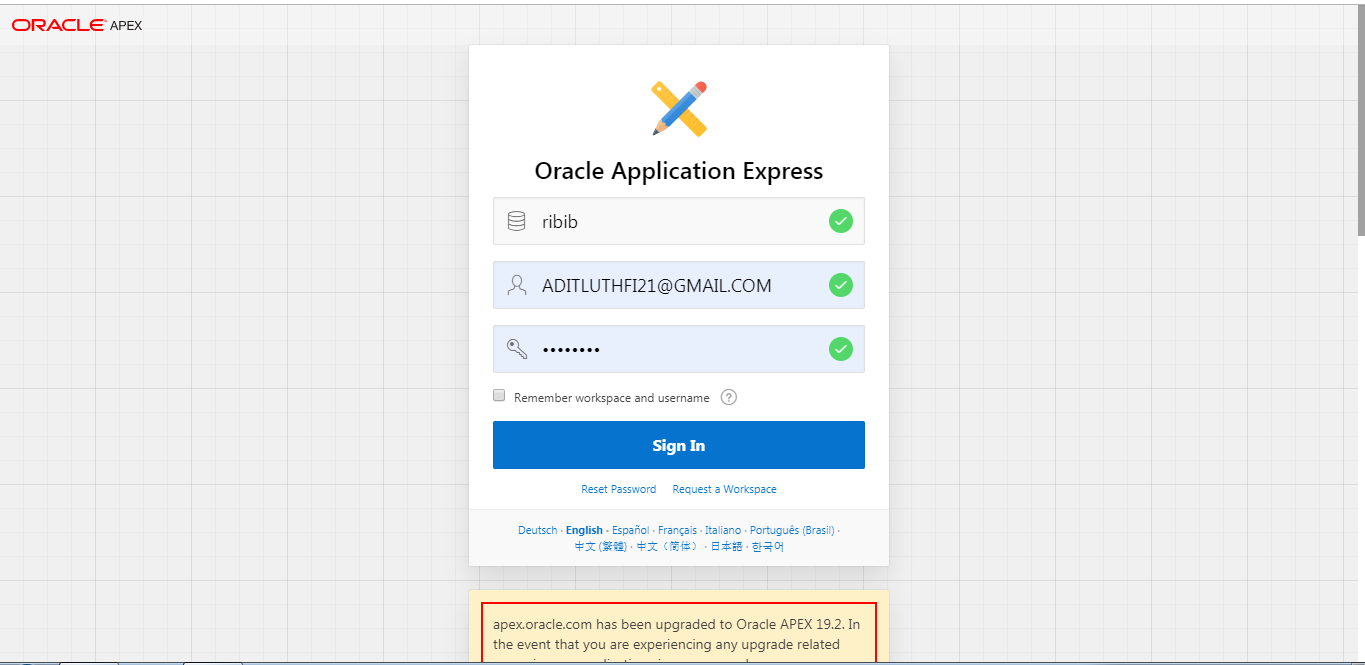
\includegraphics[scale=0.3]{gambar/1}
\end{figure}

\item Klik App builder
\begin{figure} [h]
	\centering
		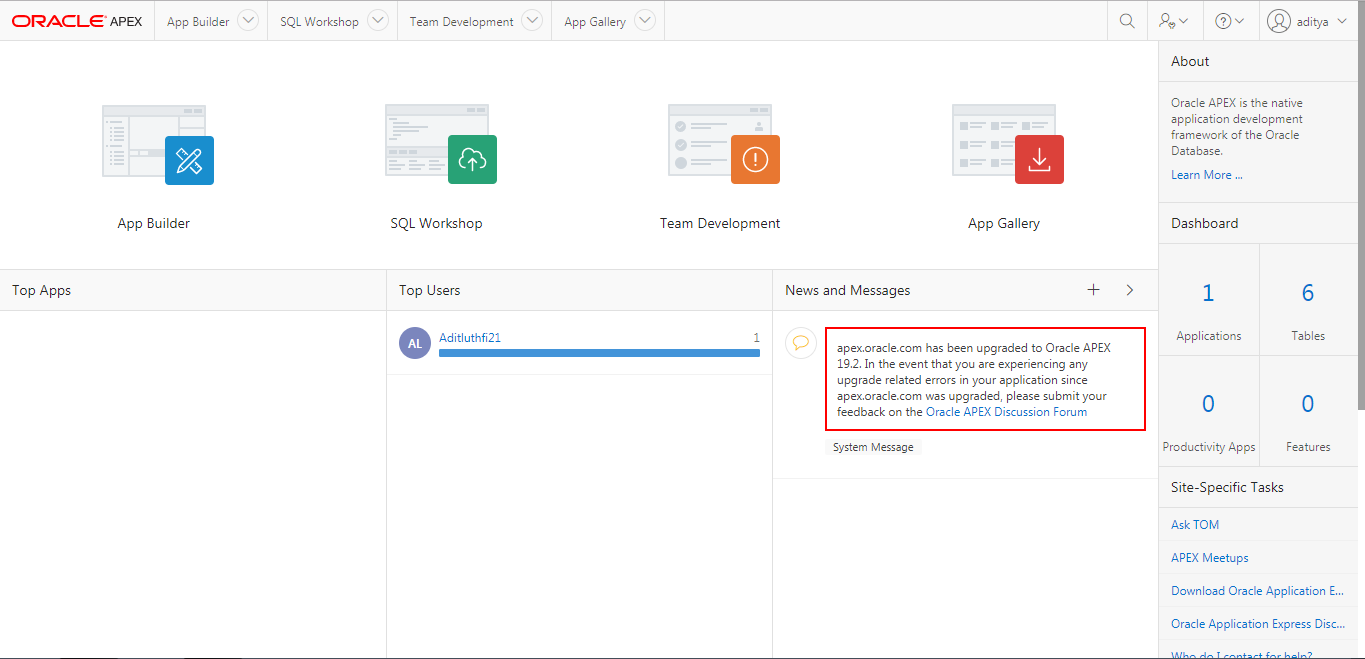
\includegraphics[scale=0.3]{gambar/2}
\end{figure}
\\
\\
\\
\item Klik Create
\begin{figure} [h]
	\centering
		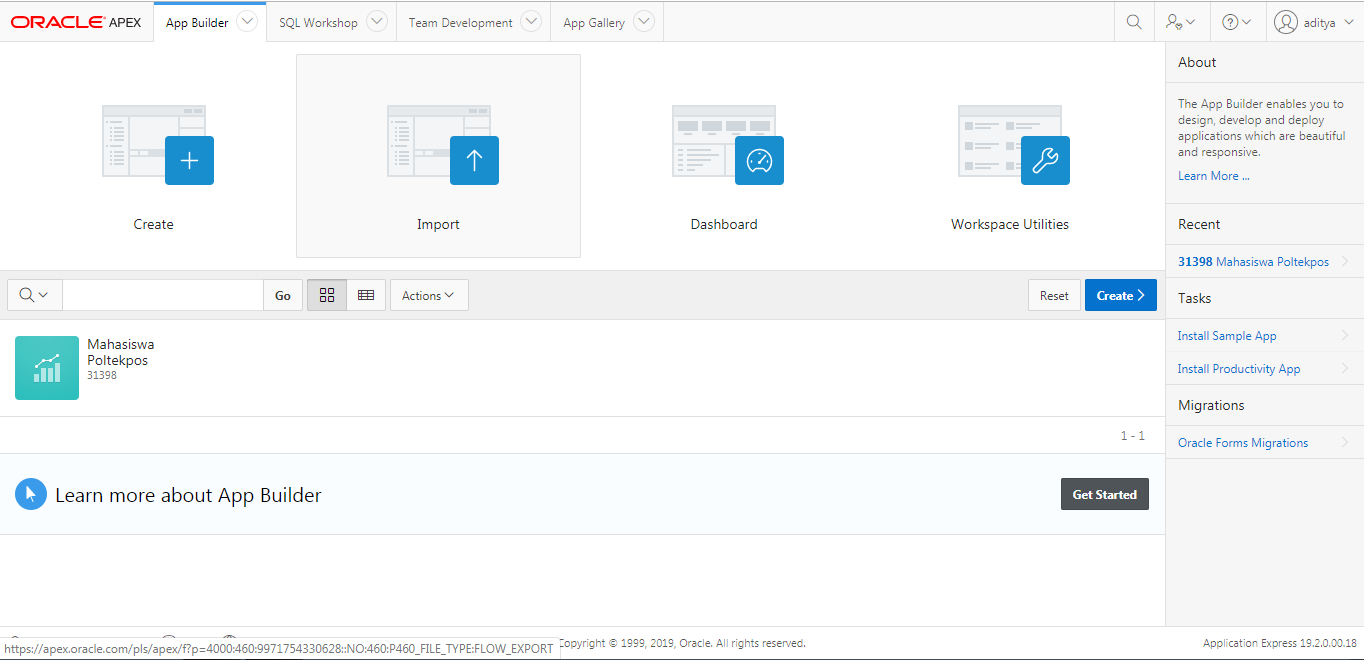
\includegraphics[scale=0.4]{gambar/3}
\end{figure}
\\
\\
\item Klik Klik From a file karena disini kita menngunakan data ang sudah ada di excel
\begin{figure} [h]
	\centering
		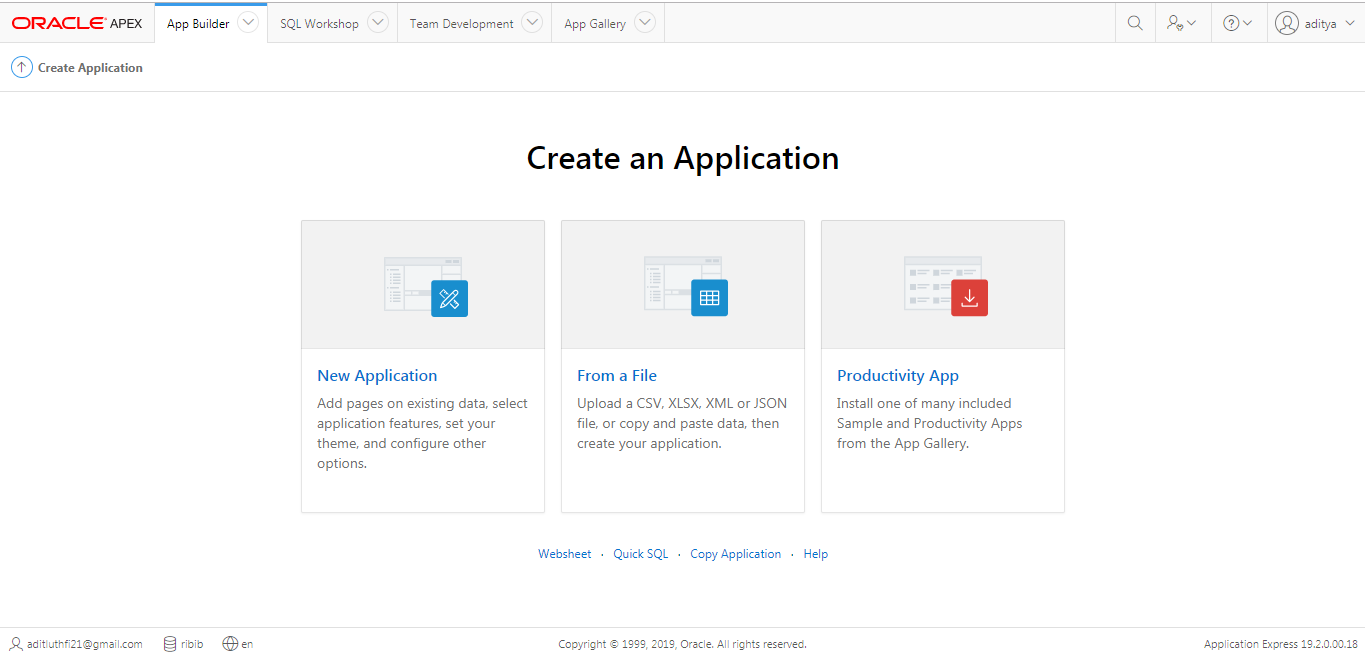
\includegraphics[scale=0.4]{gambar/4}
\end{figure}

\item Masukkan file excel anda lalu buat nama table dan jangan lupa perhatikan jika anda menggunakan 1 file excel pilihlah sheet yang sesuai dengan tablenya
\begin{figure} [h]
	\centering
		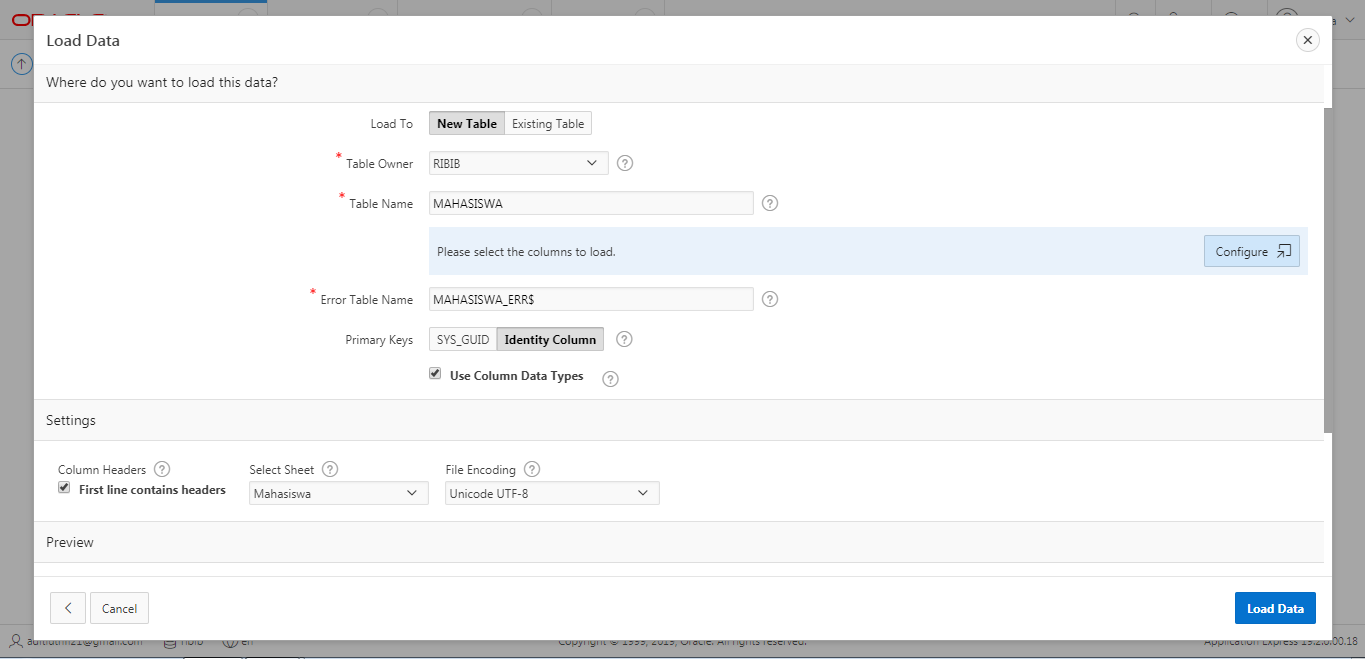
\includegraphics[scale=0.4]{gambar/5}
\end{figure}

\item Jika sudah memasukkan semua table klik SQL Workshop
\begin{figure} [h]
	\centering
		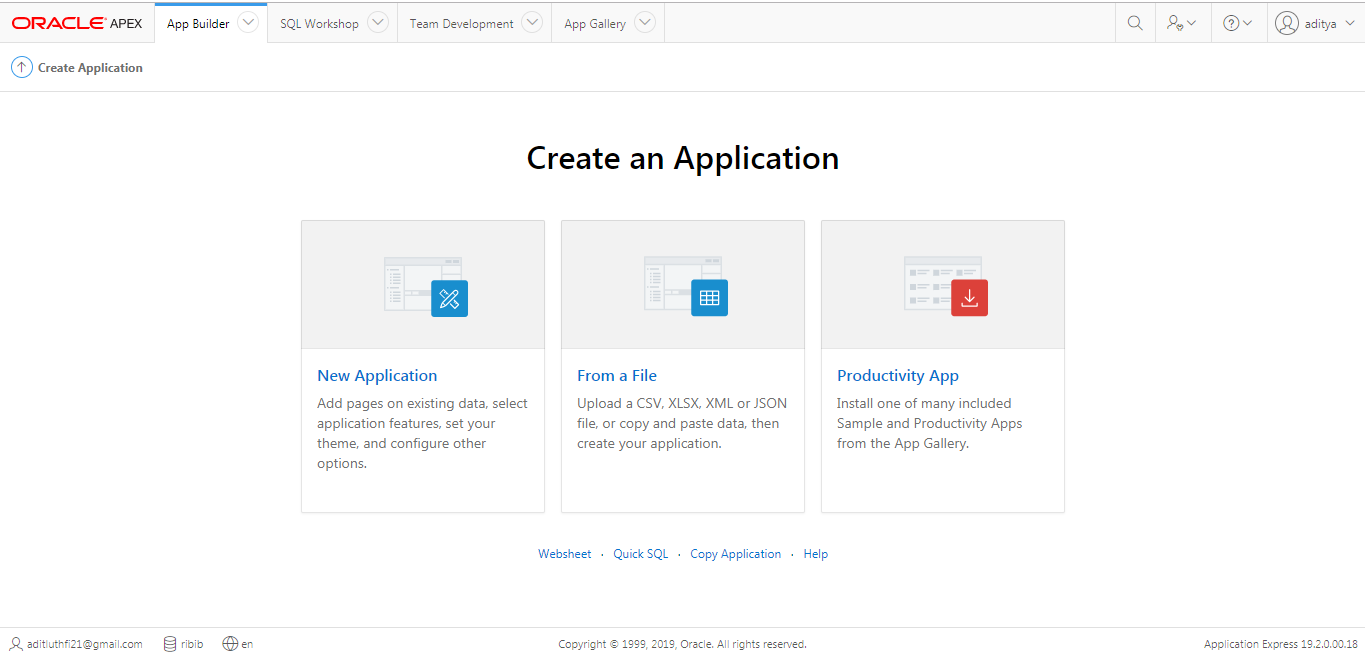
\includegraphics[scale=0.4]{gambar/4}
\end{figure}
\\
\\
\\
\\
\item Lalu klik Object Browser Untuk merubah Struktur atribut pada table yang telah kita buat
\begin{figure} [h]
	\centering
		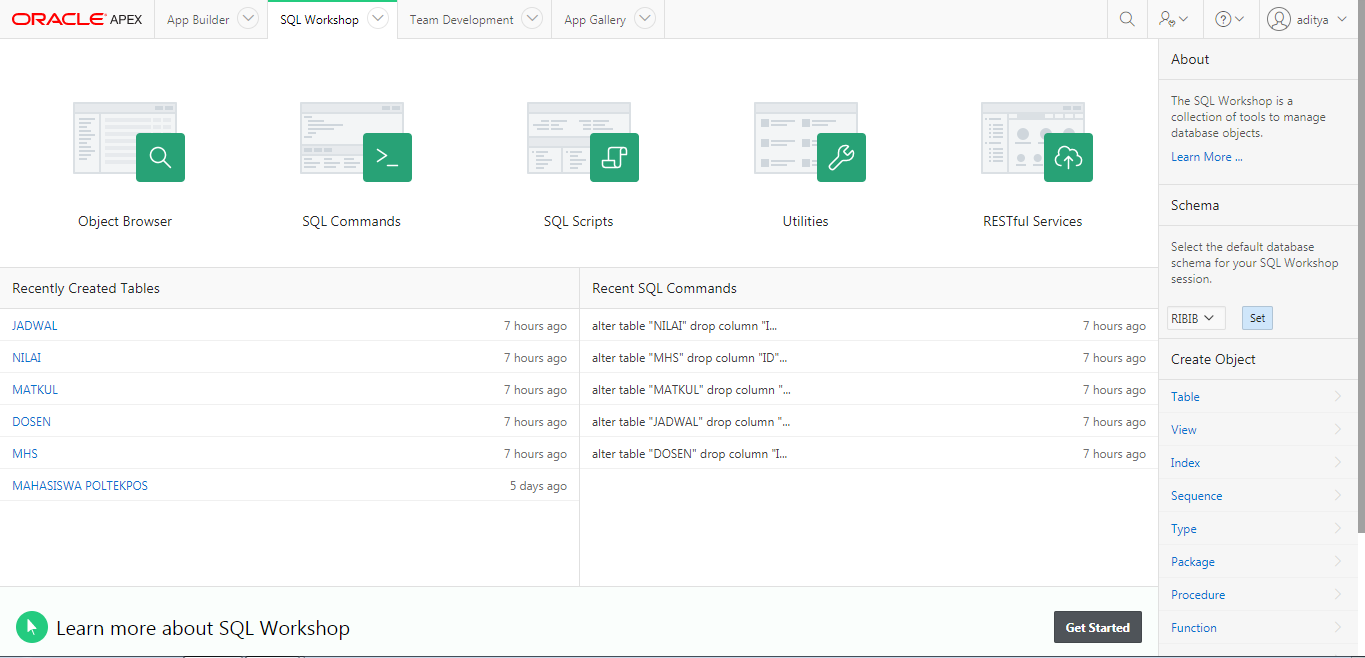
\includegraphics[scale=0.4]{gambar/6}
\end{figure}
\\
\\
\\
\item Lalu perhatihan setiap atribut pada setiap table. UNtuk memodifikasi atribut pada table klik modify column
\begin{figure} [h]
	\centering
		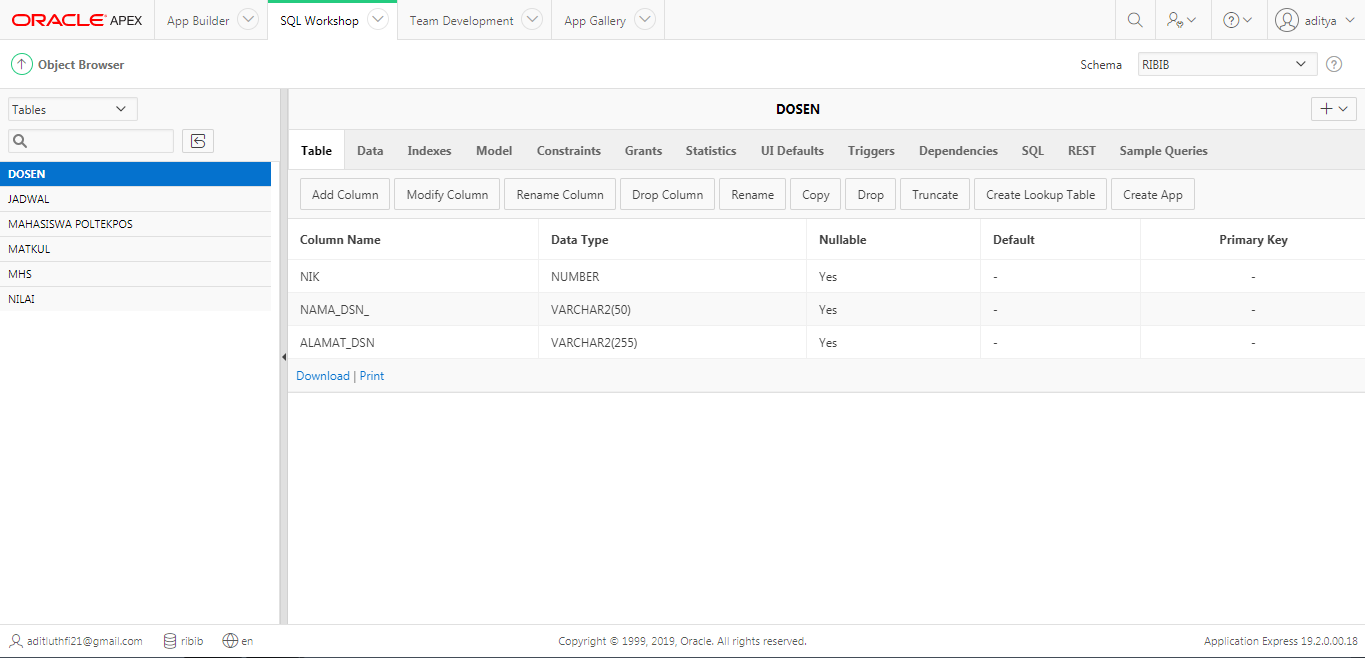
\includegraphics[scale=0.4]{gambar/7}
\end{figure}
\\
\\
\\
\\
\\
\item Buatlah setiap atribut wajib untuk di isi agar tidak ada record yang kosong
\begin{figure} [h]
	\centering
		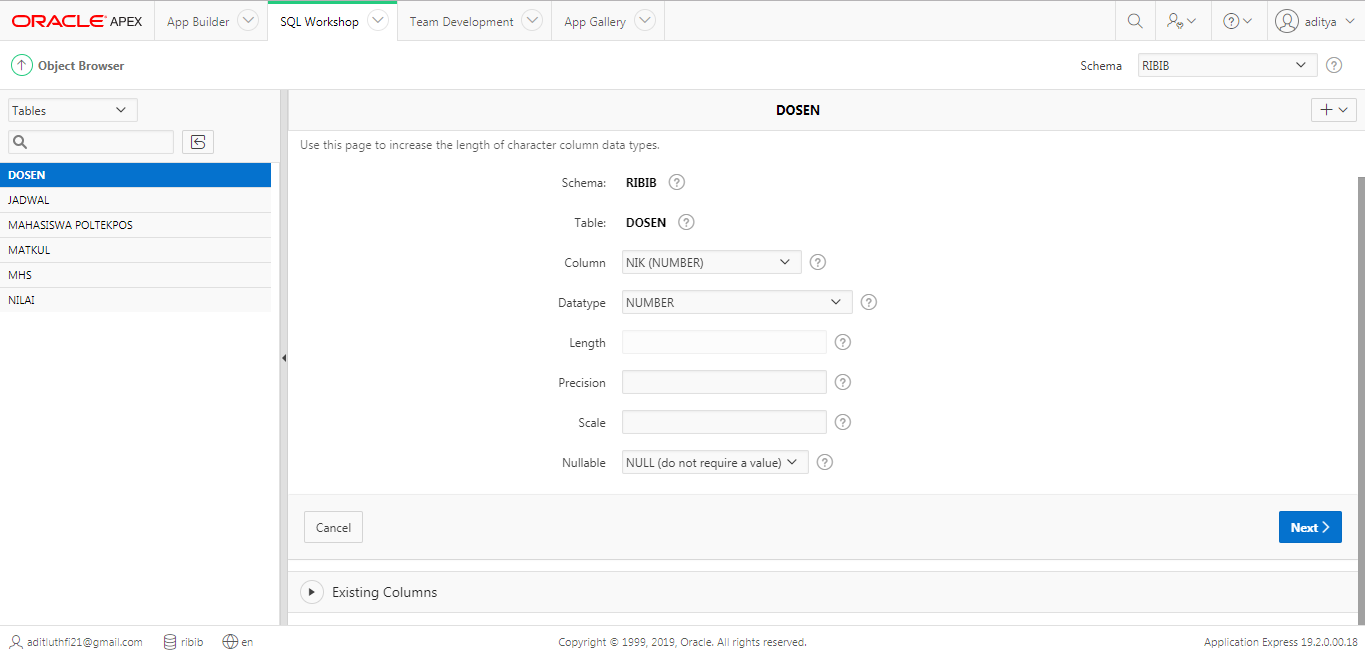
\includegraphics[scale=0.3]{gambar/8}
\end{figure}

\item Lalukakan langkah di atas untuk setiap atribut pada table yang kita buat

\item Jika semua atribut di setiap table sudah ber tipe not null maka kita buatkan primary key table yang sudah kita buat 

\item Klik SQL Workshop Lalu klik SQL Command
\begin{figure} [h]
	\centering
		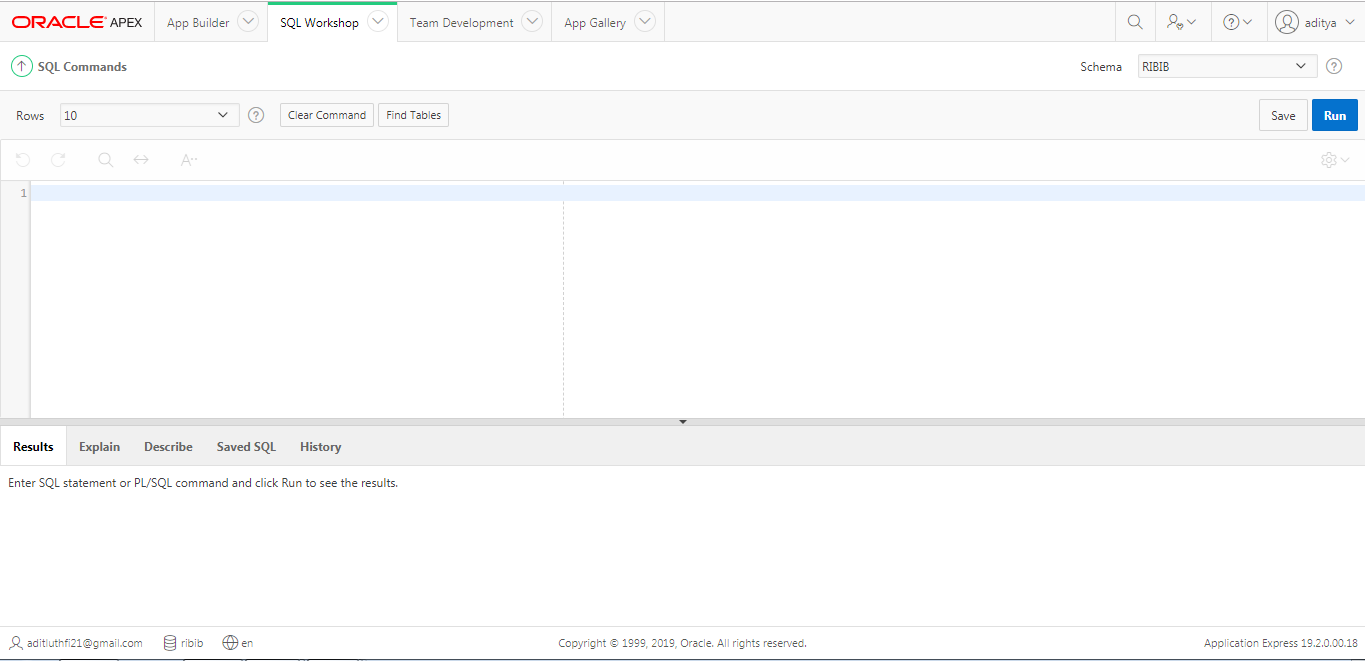
\includegraphics[scale=0.3]{gambar/9}
\end{figure}
\\
\\
\\
\\
\\
\item langkah ini untuk menciptakan primary key pada atribut NIK di table DOSEN, Lalu Klik run
\begin{figure} [h]
	\centering
		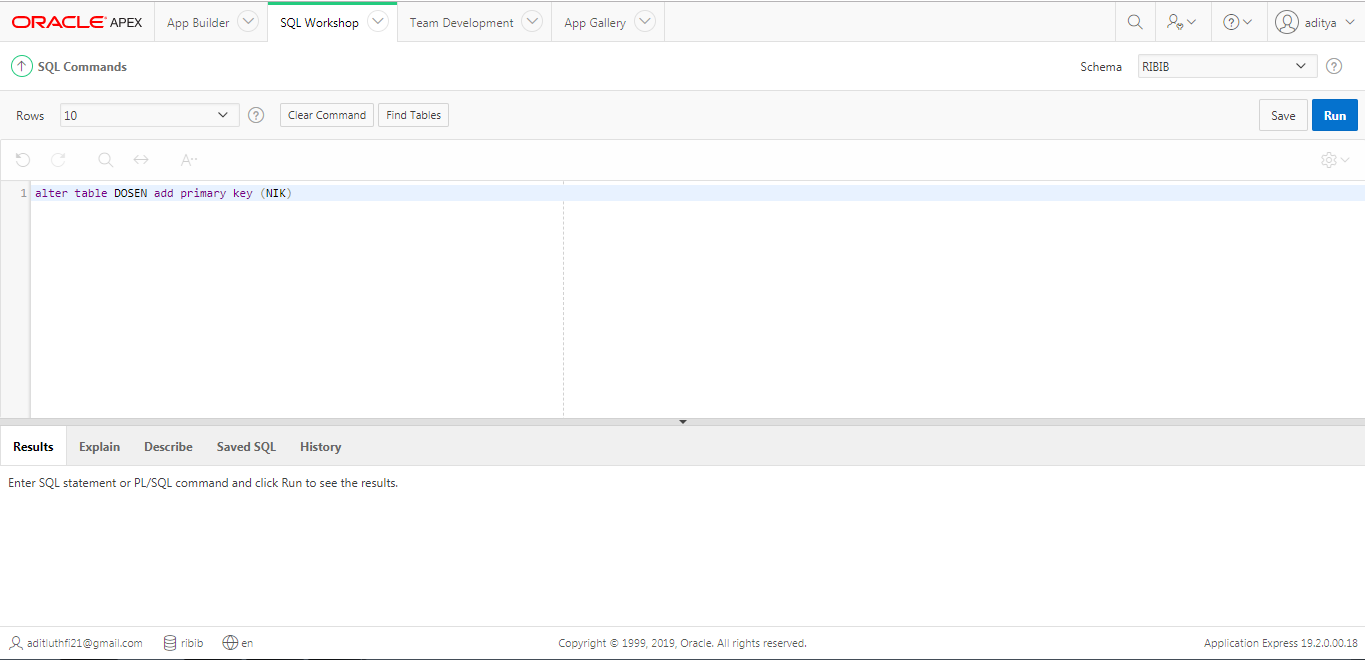
\includegraphics[scale=0.4]{gambar/10}
\end{figure}

\item langkah ini untuk menciptakan primary key pada atribut NIM di table MHS, Lalu Klik run 
\begin{figure} [h]
	\centering
		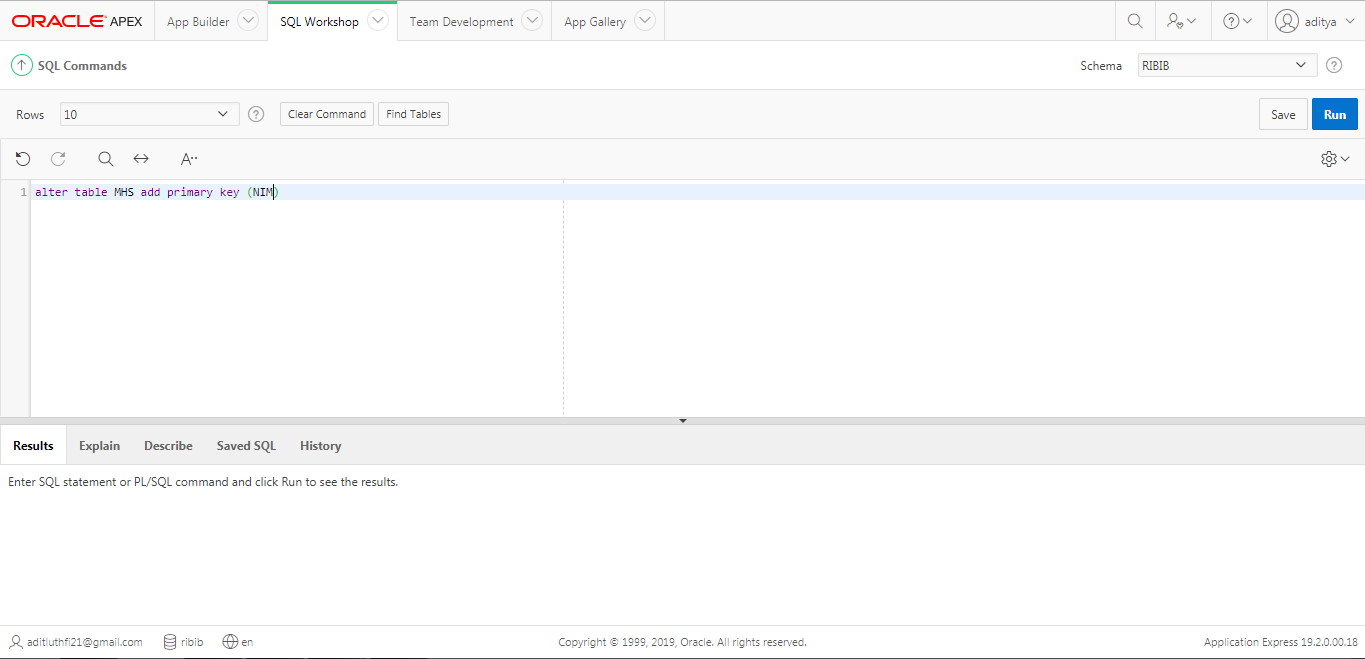
\includegraphics[scale=0.4]{gambar/11}
\end{figure}
\\
\\
\\
\\
\item langkah ini untuk menciptakan primary key pada atribut KODE di table MATKUL, Lalu Klik run 
\begin{figure} [h]
	\centering
		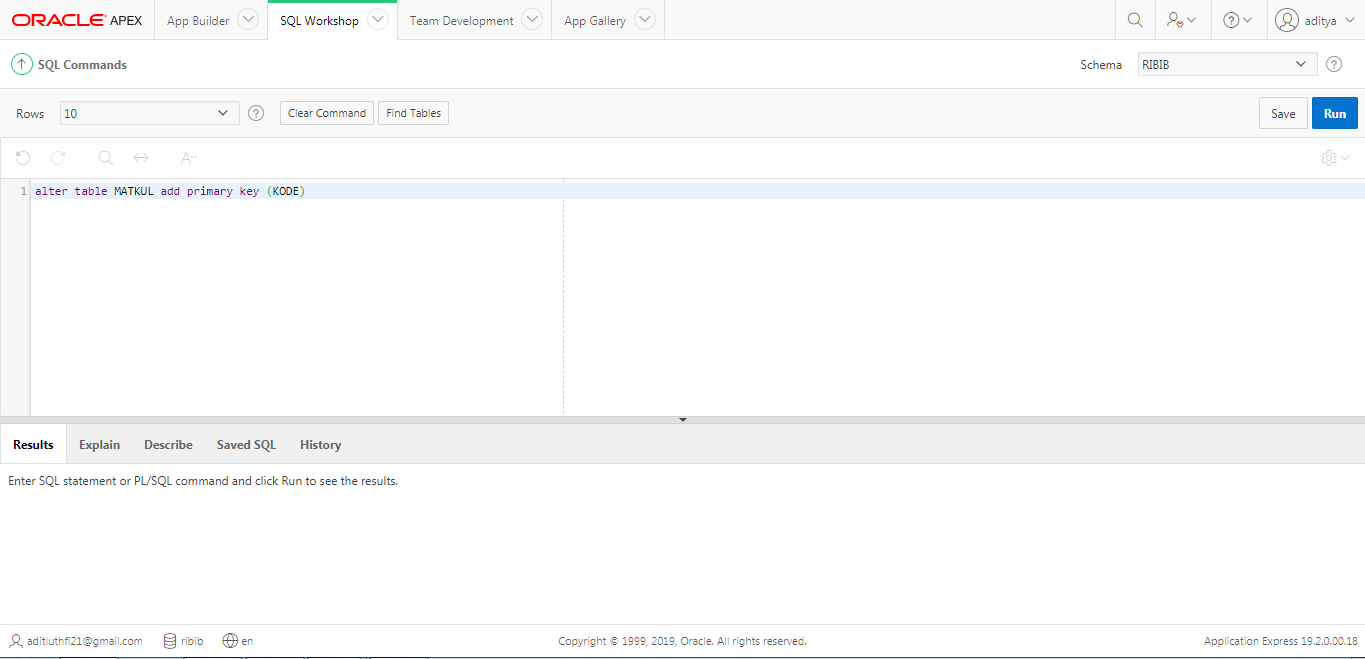
\includegraphics[scale=0.4]{gambar/12}
\end{figure}

\item langkah ini untuk menciptakan Foregen key pada atribut KODE di table JADWAL Reverensi dari atribut KODE pada table MATKUL , Lalu Klik run 
\begin{figure} [h]
	\centering
		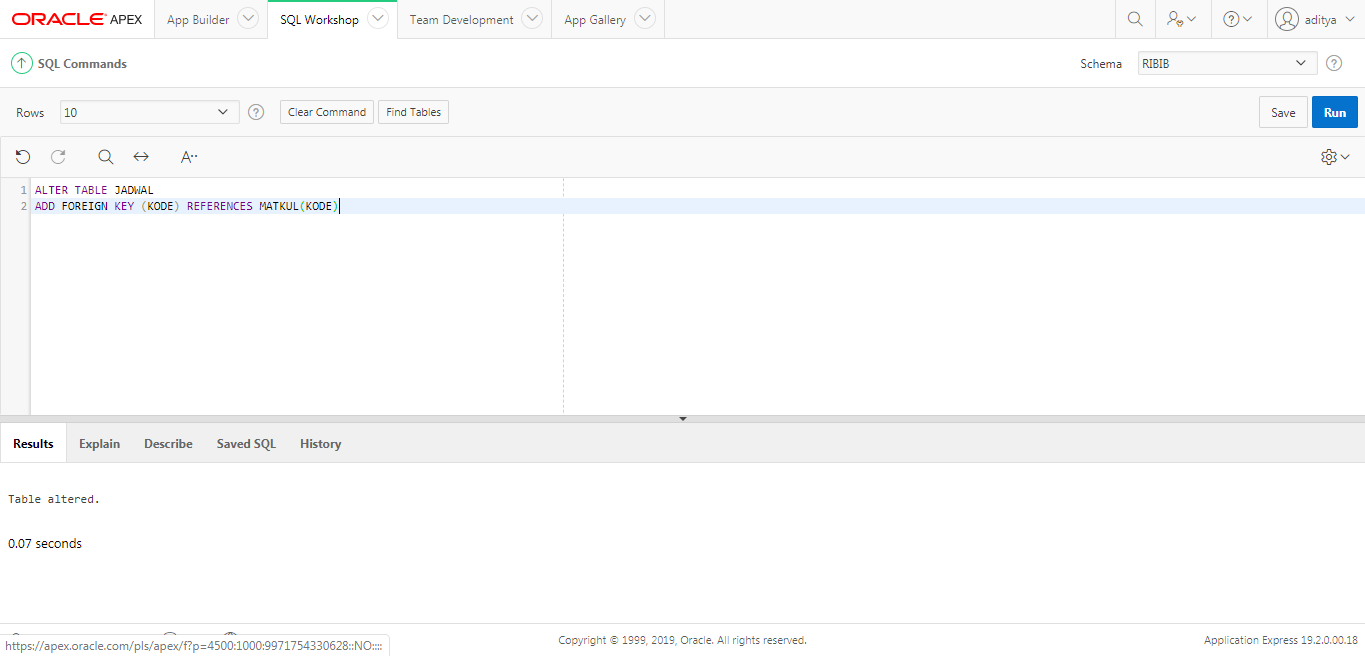
\includegraphics[scale=0.4]{gambar/13}
\end{figure}
\\
\\
\\
\\
\item langkah ini untuk menciptakan Foregen key pada atribut KODE di table NILAI Reverensi dari atribut KODE pada table MATKUL , Lalu Klik run 
\begin{figure} [h]
	\centering
		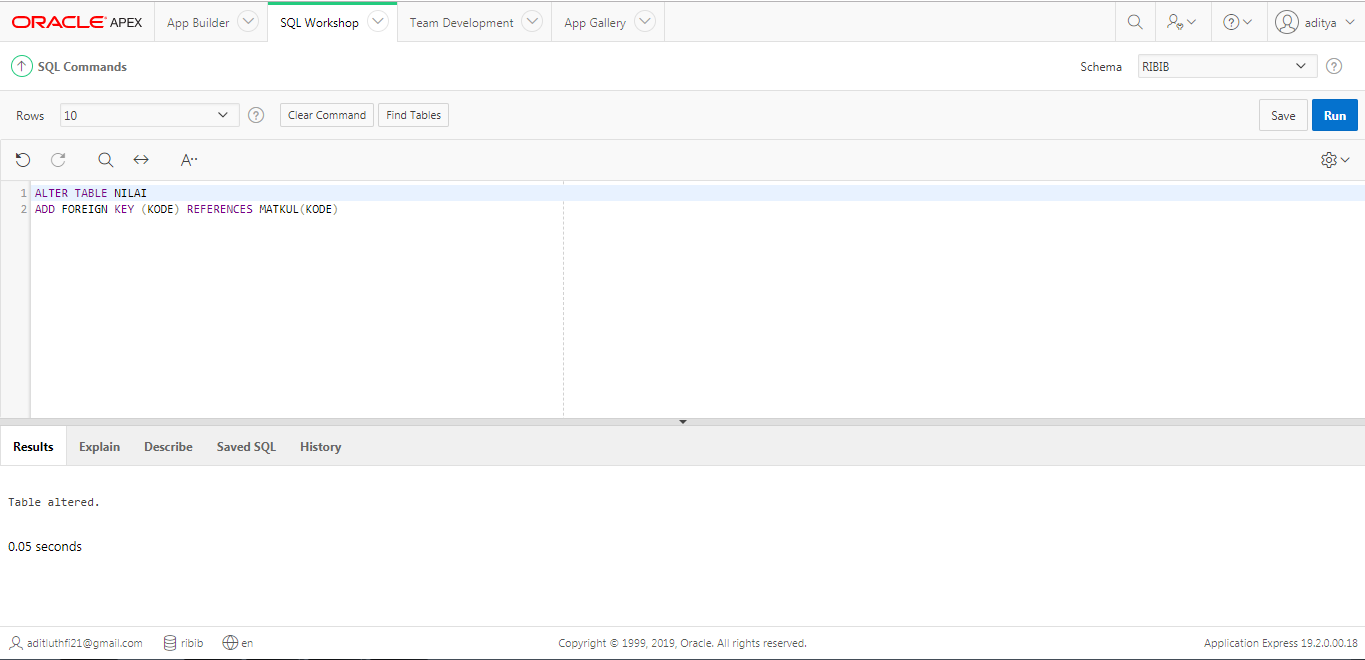
\includegraphics[scale=0.4]{gambar/14}
\end{figure}

\item Setelah kebutuhan table telah terpenuhi, selanjutnya dalah membuatkan aplikasi dari table-table tersebut

\item Klik App builder, lalu klik Create
\begin{figure} [h]
	\centering
		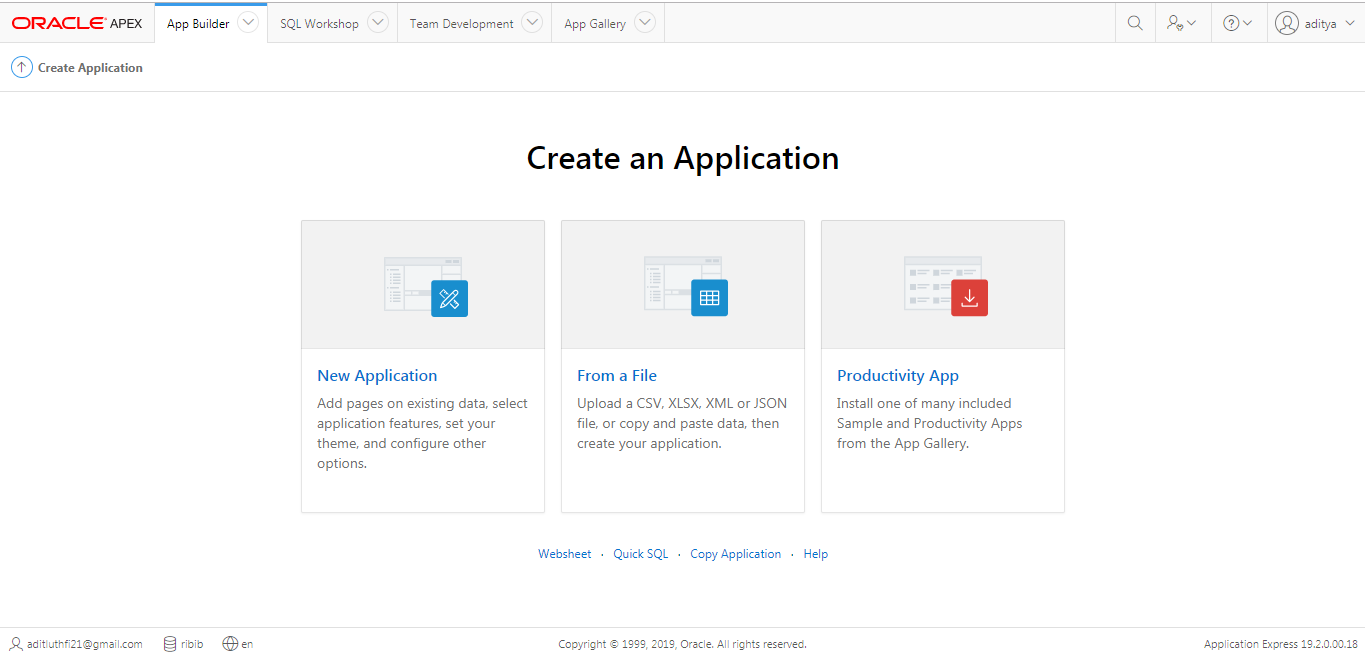
\includegraphics[scale=0.4]{gambar/4}
\end{figure}
\\
\\
\\
\\
\item Lalu Klik New Aplication
\begin{figure} [h]
	\centering
		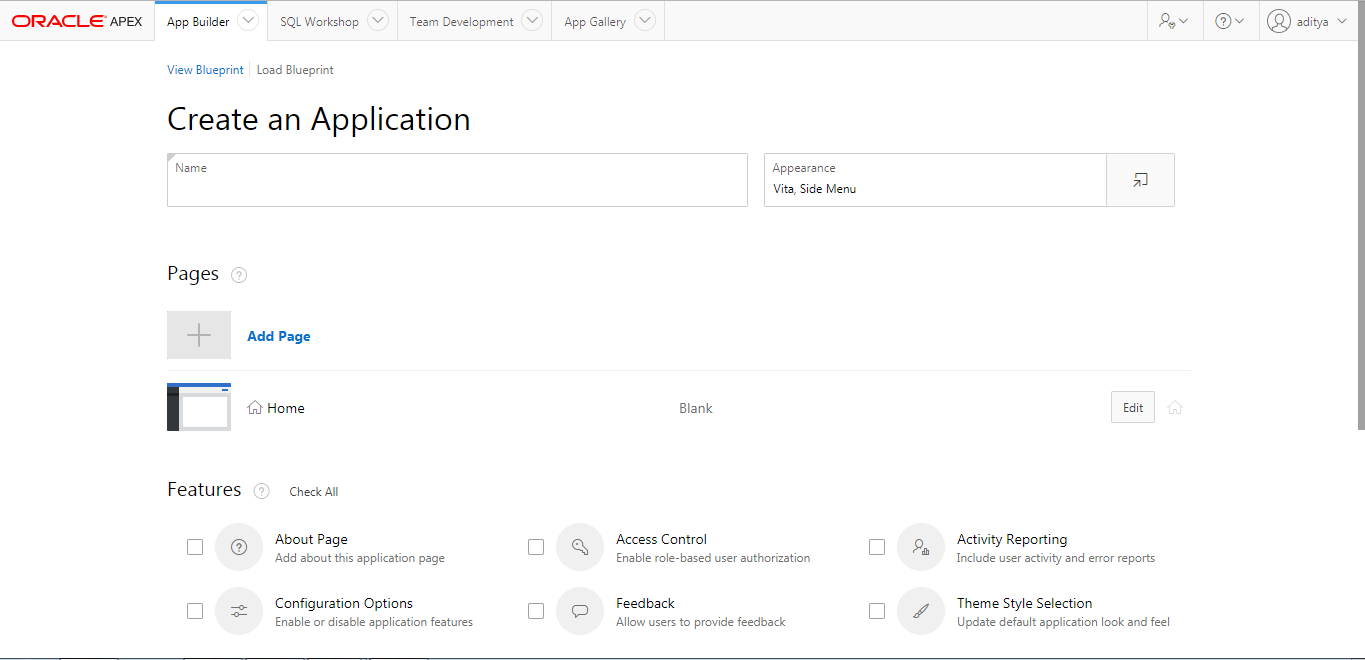
\includegraphics[scale=0.4]{gambar/15}
\end{figure}

\item Lalu isi Nama Aplikasi yang ingin di buat berdasarkan Table yang sudsh kita normalisasi

\item Lalu klik Add Page sesuai kebutuhan(saya disini menggunakan Interactive Report)
\begin{figure} [h]
	\centering
		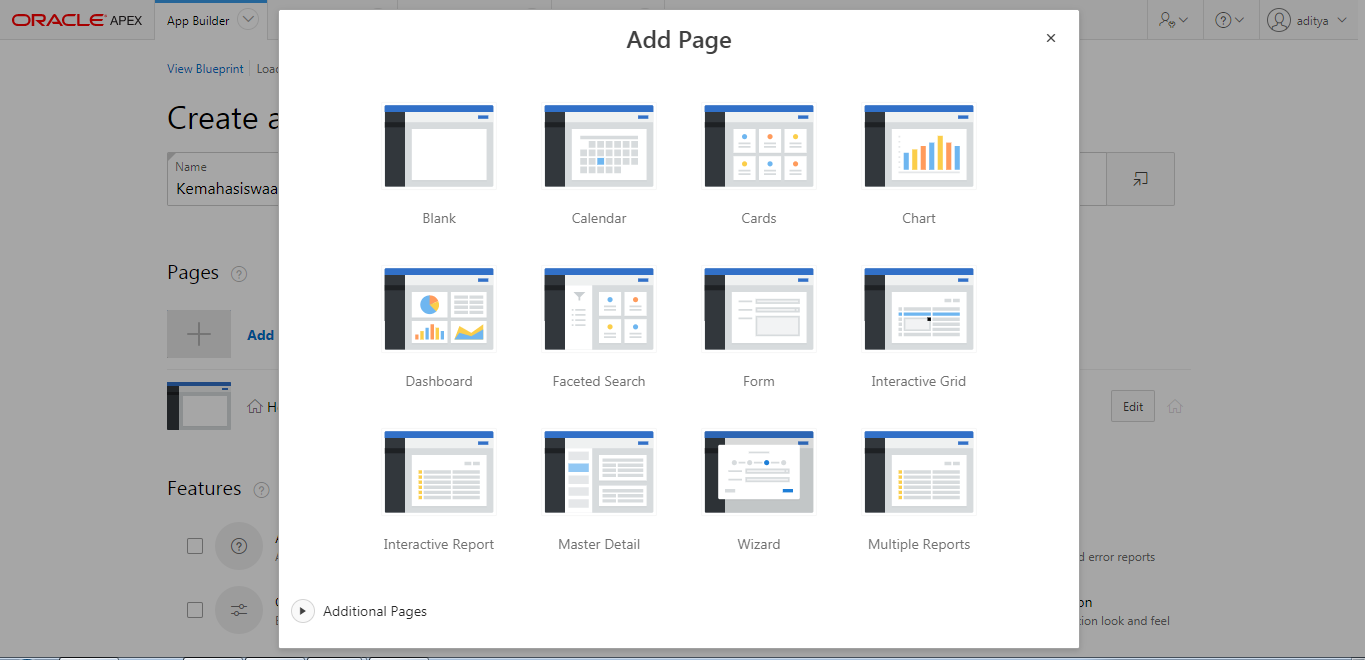
\includegraphics[scale=0.4]{gambar/16}
\end{figure}
\\
\\
\\
\\
\item Sesuaikan nama page nya dengan nama table yang dipilih
\begin{figure} [h]
	\centering
		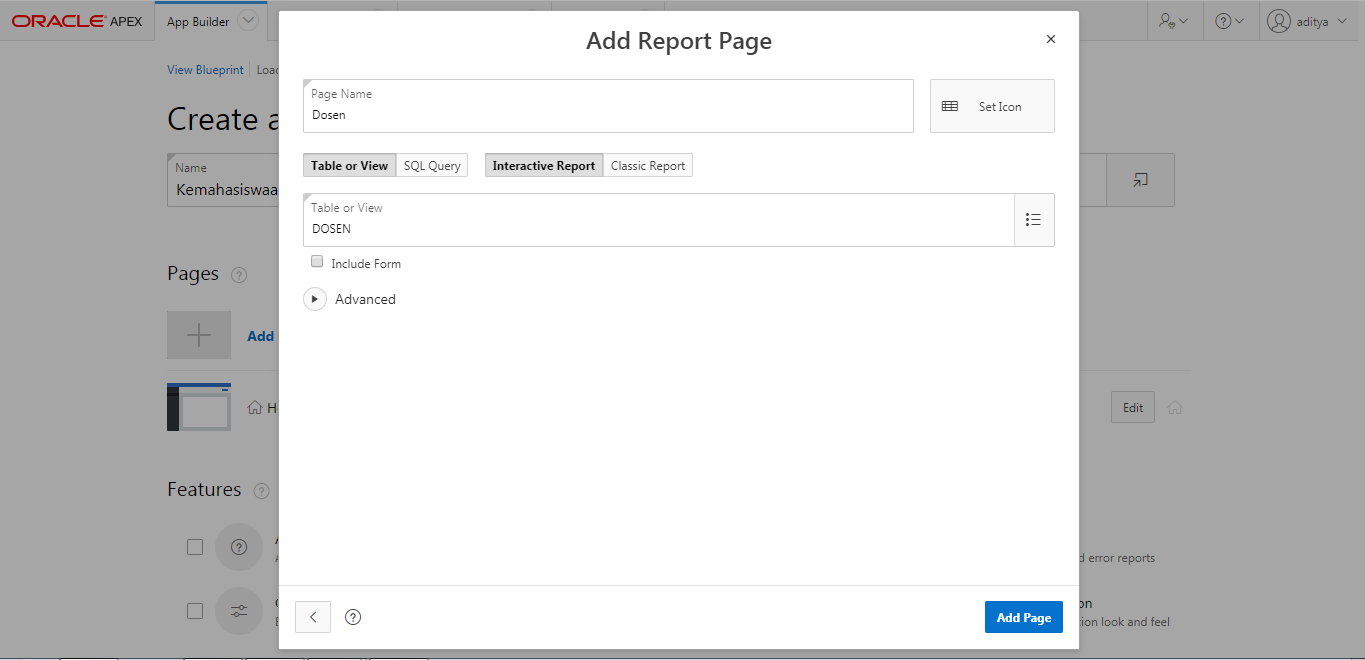
\includegraphics[scale=0.4]{gambar/17}
\end{figure}

\item Lalukan langkah di atas untuk semua table yang telah di normalisasikan

\item Jika semua page yang berisi table telah di buat
\begin{figure} [h]
	\centering
		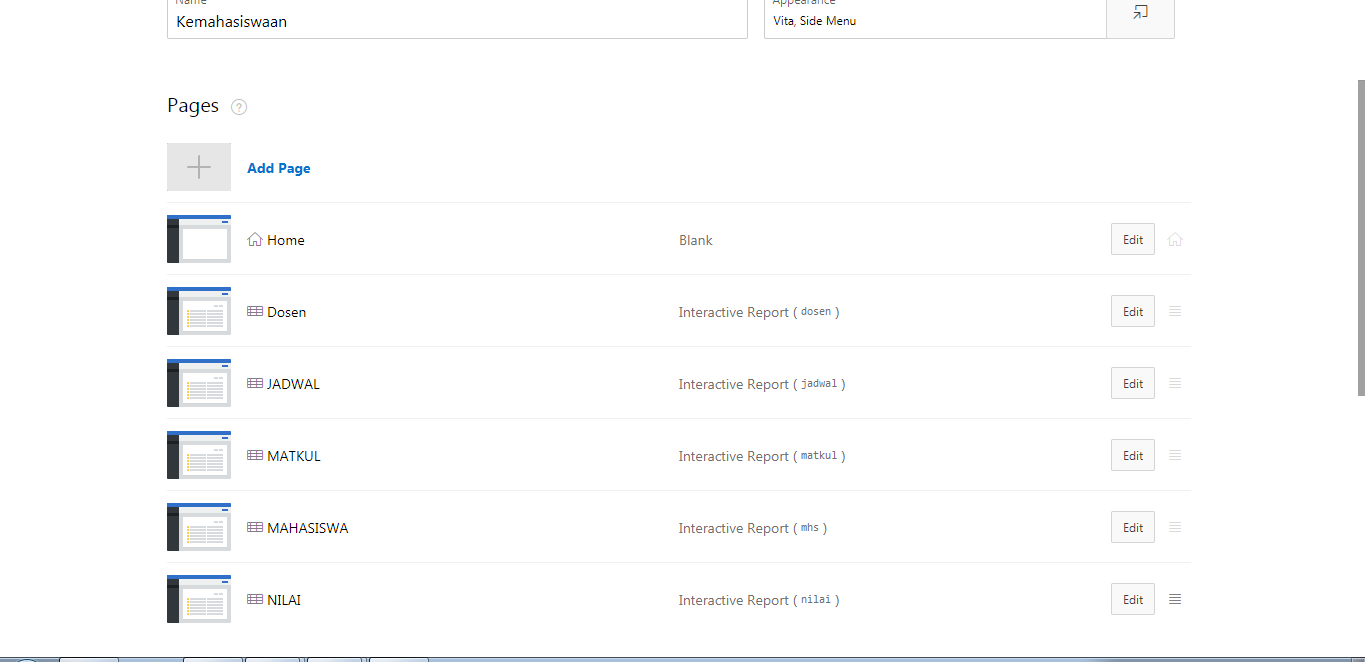
\includegraphics[scale=0.4]{gambar/18}
\end{figure}
\\
\\
\\
\\
\item Selanjutnya adalah klik Create Application
\begin{figure} [h]
	\centering
		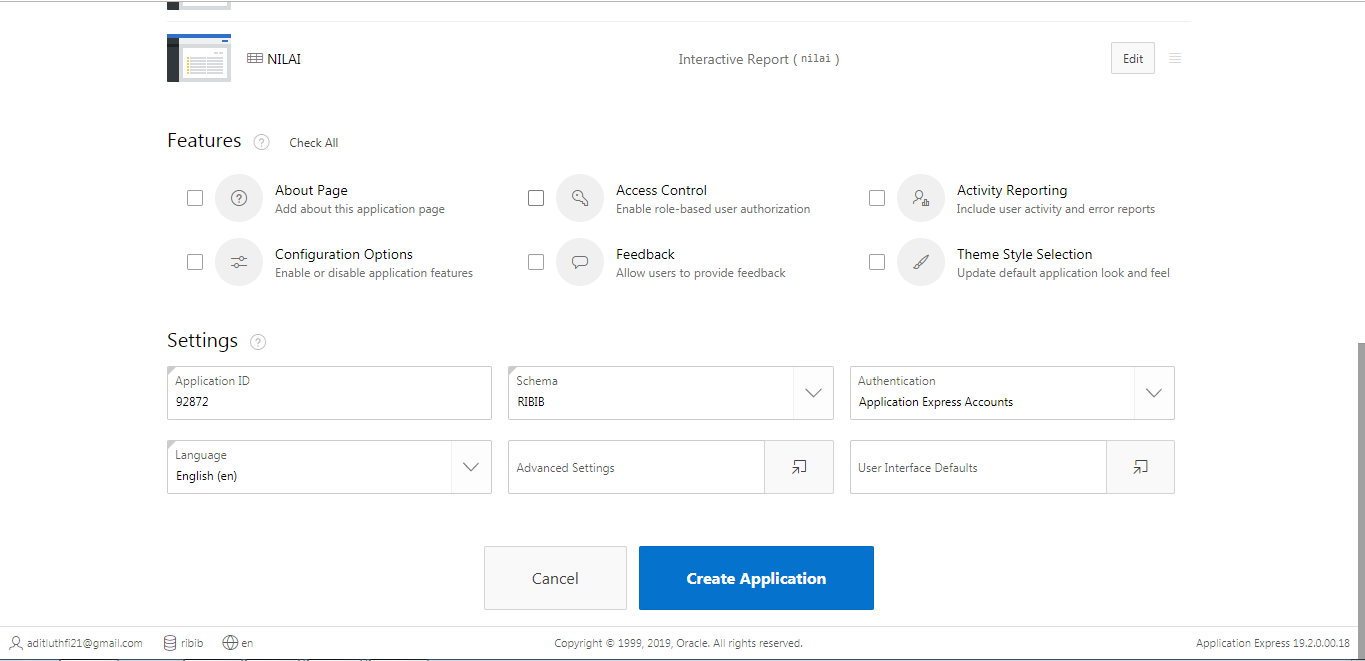
\includegraphics[scale=0.4]{gambar/19}
\end{figure}

\item Jika Loading telah selesai maka aplikasi anda telah selesai dibuat

\item Selanjutnya klik Run Application untuk memulai aplikasi yang telah di buat
\begin{figure} [h]
	\centering
		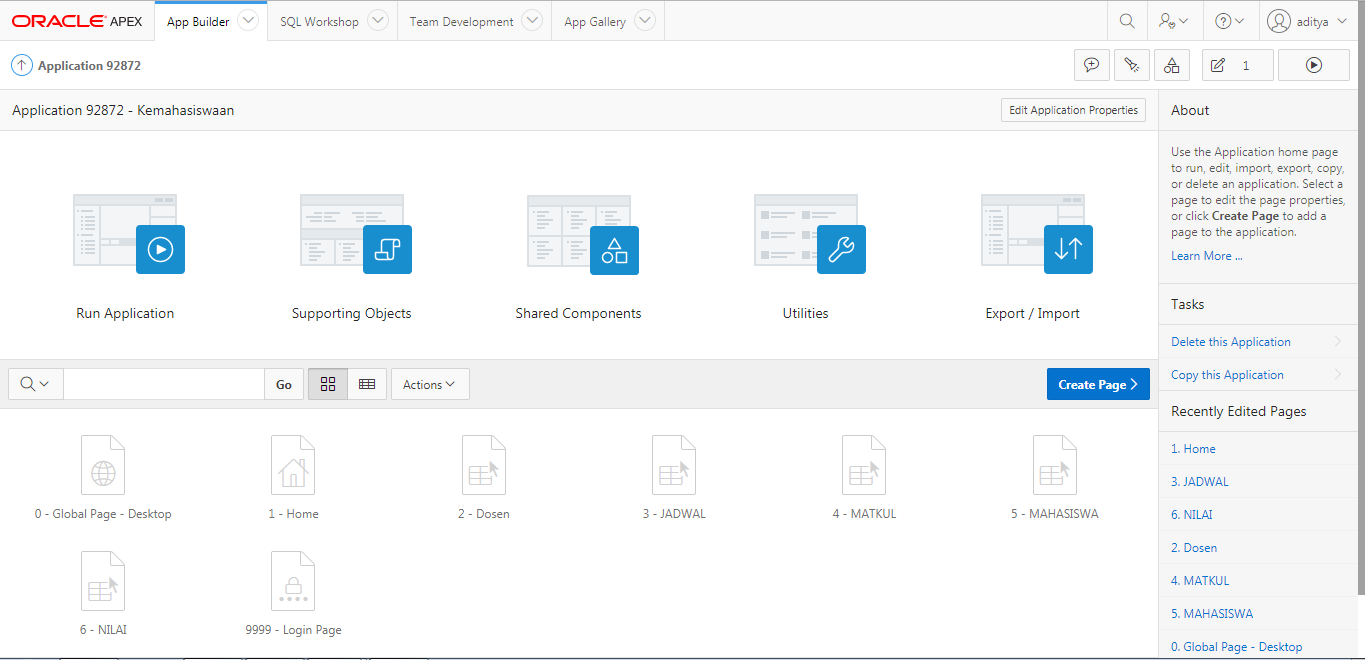
\includegraphics[scale=0.4]{gambar/20}
\end{figure}
\\
\\
\\
\\
\item Masukkan e-mail dan password anda untuk menjalankan aplikasi 
\begin{figure} [h]
	\centering
		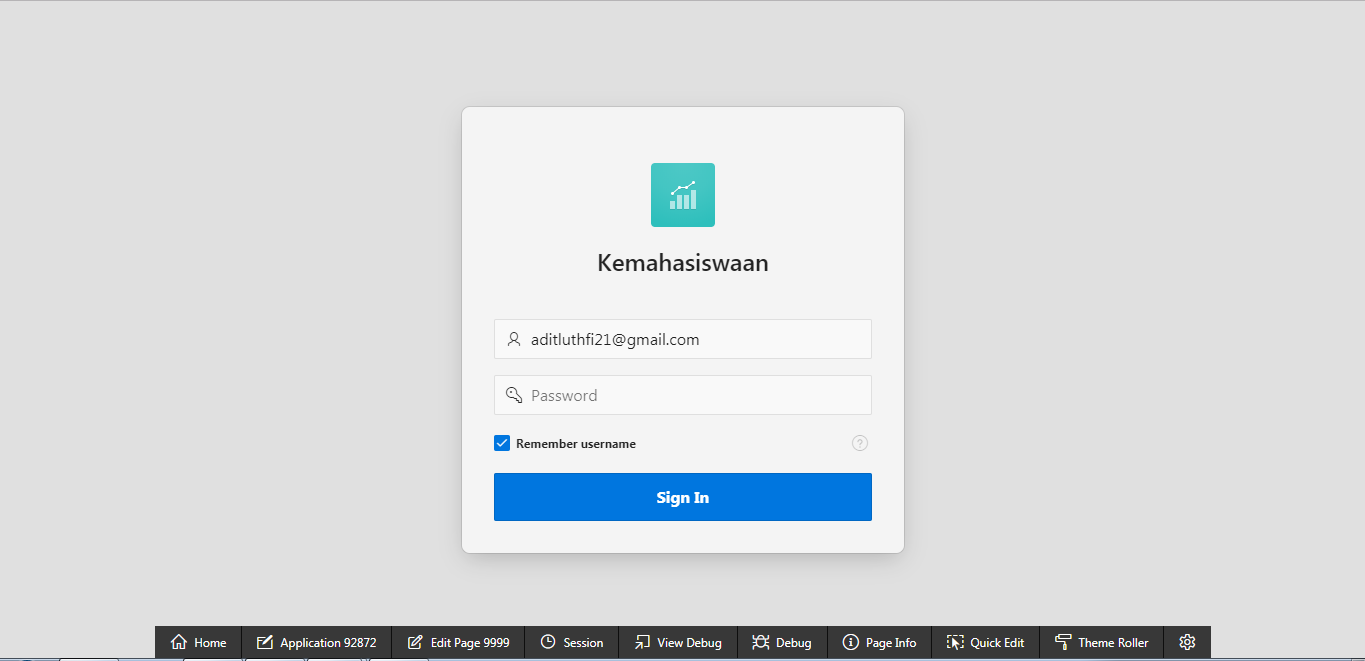
\includegraphics[scale=0.4]{gambar/21}
\end{figure}

\item Aplikasi siap digunakan
\begin{figure} [h]
	\centering
		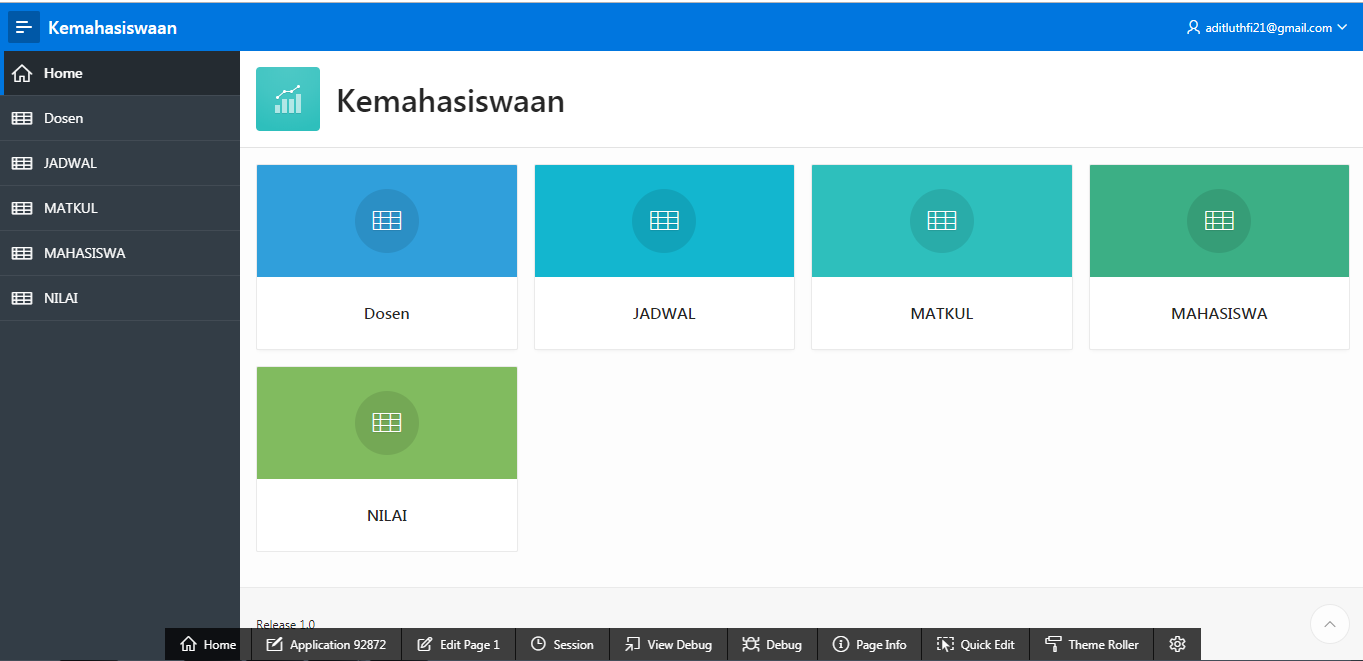
\includegraphics[scale=0.4]{gambar/22}
\end{figure}

\end{enumerate}

\section*{Untuk Login aplikasi silahkan gunkan}
\begin{enumerate}
\item workspace ribib
\item email ADITLUTHFI21@GMAIL.COM
\item password ribib021
\item link aplikasi\\ 
https://apex.oracle.com/pls/apex/f?p=92872:LOGIN\textunderscore DESKTOP:16366338962381:::::
\end{enumerate}




\end{document}